
\chapter{Software-Tests und Debugging} \label{sec:test}
% testbackend muss noch geschrieben werden
% überlegungen zum testen aufschreiben 
Bei \ac{ARRI} gibt es drei Testebenen für die Kameras. Zunächst obliegt das Testen den Softwareentwicklern, welche durch eigene Unittest einzelne Bestandteile ihrer Implementierung testen. Bei einem erfolgreichen Unittest wird von dem Entwickler ein funktionaler Integrationstest auf der Kamera durchgeführt. Hierzu werden die eigenen Änderungen in der Software kompiliert und auf die Kamera geladen und vor allem die geänderten Funktionalitäten getestet. Die letzte und ausführlichste Ebene findet bei einem Testteam statt. Dort wird die Software nicht nur im Bezug auf die Änderungen geprüft, sondern auch die allgemeine Funktionsfähigkeit der Kamera getestet und festgestellt.


\section{Einführung}
Zum Testen der Funktionalität der Software haben sich über die Zeit Grundsätze gebildet, welche als generelle Leitlinien beim Testen gesehen werden. \citep[S. 53]{spillner2005basiswissen}
Einige Grundsätze sollen im Folgenden näher betrachet werden, weil sie für den Frameworktests essentiell sind. 

Der erste Grundsatz besagt, dass ausreichendes Testen die Wahrscheinlichkeit von Fehlern im laufenden Betrieb verringert. Das Ausbleiben von Fehlern beim Testen ist kein Indikator für die Fehlerfreiheit des Codes.
Im zweiten Grundsatz wird erläutert, dass vollständiges Testen nicht möglich ist. Eine Ausnahme sind die Tests bei sehr trivialen Testobjekten. 
Für die frühzeitige Erkennung der Fehler besagt der dritte Grundsatz, dass frühzeitig mit dem Testen begonnen werden soll. \citep[S. 53]{spillner2005basiswissen}


Vor allem durch den zweiten Grundsatz wird klar, das es nicht möglich ist, dass komplette \gls{framework} zusammen zu testen. Um einfache Testobjekte zu erhalten, werden die einzelnen Module über die \ac{fra}-Bibliothek getestet. Durch die Unittest der Module wird zudem die Wahrscheinlichkeit von Fehlern in diesem Bereich verringert. Außerdem sollen die Tests entsprechend mit neuen Funktionen in der Bibliothek erweitert werden um Fehler frühzeitig zu erkennen.


Durch die \gls{unittest} können nicht alle potenziellen Fehlerfälle abgedeckt werden. Durch die Abhängigkeit der korrekten Funktionsweise der Kamera von allen Prozessen, ist einfaches Debugging nicht möglich. In der Software wird die Fehlersuche bereits über die Protokollierung von Meldungen in einer Datei gehandhabt. Um eine schnelle und einfache Möglichkeit zu bieten, die Zugriffe im \ac{fra} zu protokollieren und eventuell neue Geräte anzulegen, wird die Funktionalität in kleine Programme eingebettet, welche im laufenden Betrieb der Kamera ausgeführt werden können.



\section{Plattformunabhängige Tests}
%Hierzu sollen die modulspezifischen Funktionen mit definierten Parametern aufgerufen werden und anschließend kontrolliert werden, ob die Funktionen die richtigen Parameter weitergibt.
Zunächst soll auf die Tests eingegangen werden, die unabhängig von der Entwicklungsumgebung durchgeführt werden können. Für jedes Modul wird ein \gls{unittest} angelegt. Dadurch kann die Funktionalität der einzelnen Module schnell überprüft und im Fehlerfall direkt gehandelt werden. Vor allem bei Änderungen an der \ac{fra}-\gls{middleware} und -Bibliothek können so vor der Inbetriebnahme auf der Kamera, Fehler gefunden und ausgebessert werden.


Für die Tests muss virtuelle Hardware angelegt werden, damit es unabhängig von der Hardware getestet werden kann. Im \gls{unittest} wird die Hardware nach dem Anlegen geöffnet und anschließend werden modulspezifische Funktionen aufgerufen und direkt danach wird ein Check durchgeführt. 
Der Ablauf eines \gls{unittest} ist in Abbildung~\ref{fig:testbackend} dargestellt und wird im Folgenden näher erläutert. Durch den Vergleich mit Abbildung~\ref{fig:sequkern} können die Änderungen zwischen Test- und Kernel-Backend gut visualisiert werden.


\begin{figure}[!hbtp]
	\centering
	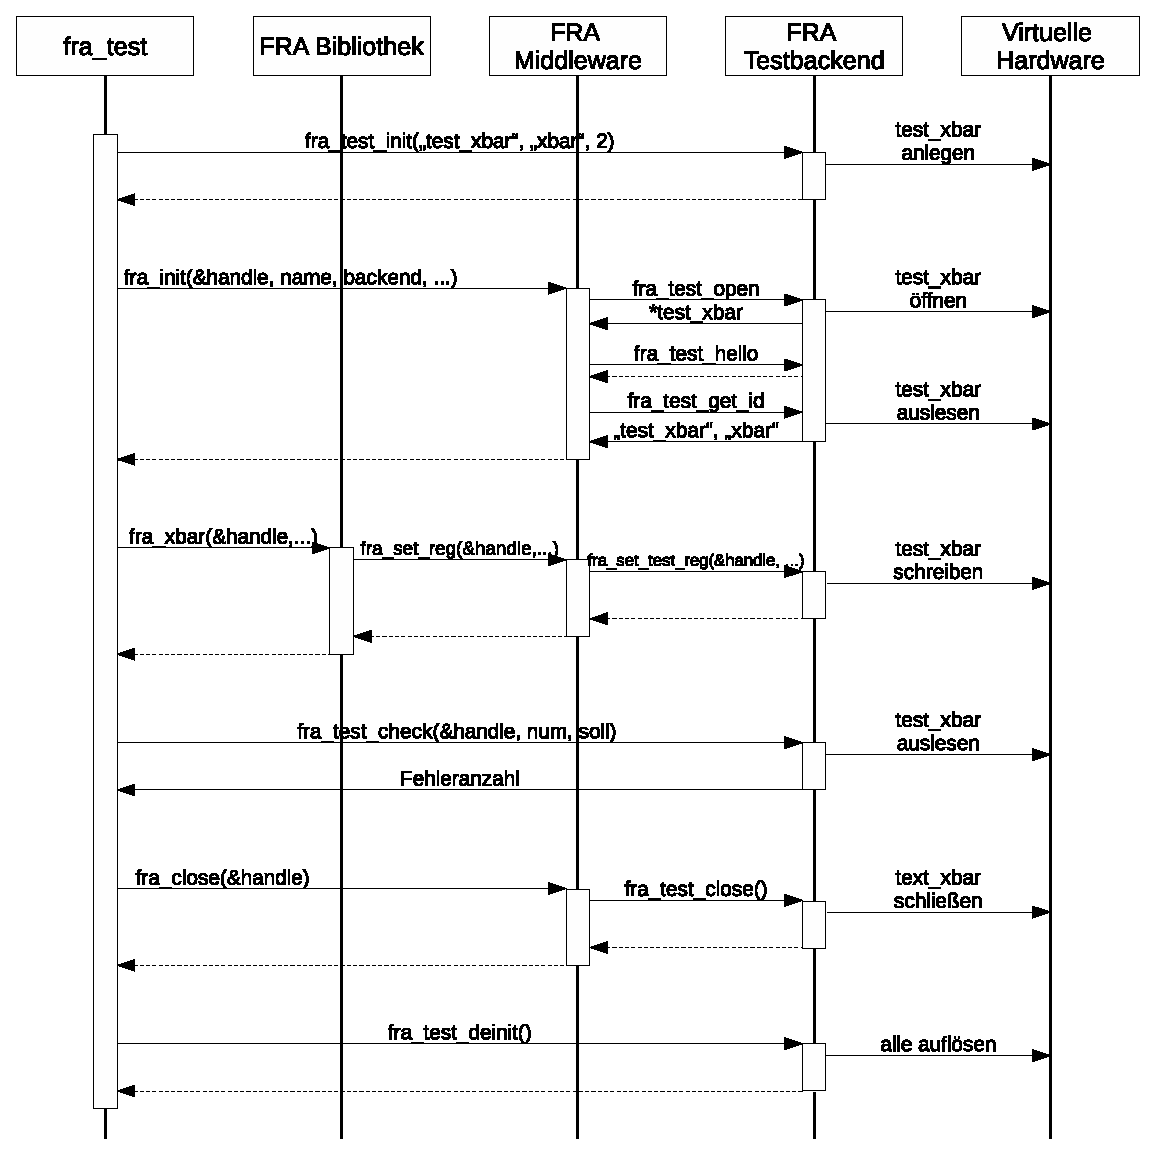
\includegraphics[width = \linewidth]{pictures/2020-01-16-testbackend.eps}
	\smallskip
	\caption{Beispielhaftes Sequenzdiagramm zum \gls{unittest}}
	\label{fig:testbackend}
\end{figure} 


Durch das Anlegen eines Geräts im Kernel-Backend können alle benötigten Informationen und Register über dieses Gerät abgefragt und gesetzt werden. Aufgrund der notwendigen Unabhängigkeit von der Hardware ist das Anlegen der Geräte im Test-Backend so nicht möglich. Um eine ähnliche Funktionalität wie im Kernel zu haben, wird das Modul über die \textit{fra\_mod\_test} Struktur abgebildet. Hier werden alle notwendigen Informationen abgelegt und auch entsprechende Register abgebildet, damit diese beschrieben und auch ausgelesen werden können.
Die \textit{fra\_mod\_test} Struktur wird als statisches Array im Test-Backend angelegt und bildet die virtuelle Hardware für das Testprogramm. Dadurch ist das Überprüfen der Register später möglich. Außerdem ist so die maximale Anzahl der Module vorgegeben. 


\begin{lstfloat}
\begin{lstlisting}
struct fra_test_mod
{
	char type[FRA_MAX_NAME];
	char name[FRA_MAX_NAME];
	uint32_t size;
	uint32_t *reg;
};
\end{lstlisting}
\captionof{code}{\label{code:fra_test_mod} Struktur zum Abbilden der virtuellen Hardware}
\end{lstfloat}

Damit die virtuelle Hardware richtig initialisiert wird, müssen für die Register entsprechender Speicherplatz allokiert, aber auch die restlichen Parameter gesetzt werden. Beim Beenden des Programms muss der Speicherbereich der Register wieder freigegeben werden. Dafür gibt es im Test-Backend zusätzliche Funktionen, durch die die Initialisierung (\textit{fra\_test\_init}) und die Deinitialisierung (\textit{fra\_test\_deinit}) durchführen.\\

 
Beim Starten des Tests werden der \textit{fra\_test\_init} Funktion drei Parameter übergeben. Zum Einen wird der Name sowie der Typ des Moduls überreicht und zum Anderen die Größe des Registers. Ist die maximale Anzahl der Module noch nicht überschritten, wird mithilfe der Größe ein Registerblock allokiert und im Anschluss wird die \textit{fra\_mod\_test} Struktur mit allen vier Parametern gefüllt und eine statische Variable \textit{mod\_count} erhöht.

Wenn der Testzyklus abgeschlossen ist, werden in der \textit{fra\_test\_deinit} Funktion mithilfe der Variablen \textit{mod\_count} alle allokierten, virtuellen Geräte wieder freigegeben.\\


Zum Öffnen eines Moduls im Test-Backend wird analog zum Kernel-Backend die Funktion \textit{fra\_init} aufgerufen. Hier wird allerdings ein anderer Backend-Typ übergeben und somit in den Wrapper-Funktionen entsprechend ins Test-Backend weitergeleitet. 
Die Funktionalität der einzelnen Backend-Funktionen ist, im Vergleich zum Kernel-Backend, vereinfacht worden und die Funktionen kommen entsprechend ohne \ac{ioctl}s aus. Das Setzen und Lesen der Register erfolgt nun über die \textit{fra\_mod\_test} Struktur im \gls{handle}. Diese wird bei der \textit{fra\_test\_open} Funktion als Zeiger auf die entsprechende Stelle im statischen \textit{fra\_mod\_test} Array angegeben. Die richtige Stelle wird über einen Vergleich mit dem Modulname gefunden.\\



Damit überprüft werden kann, ob die Register richtig beschrieben bzw. ausgelesen worden sind, gibt es zwei Funktionen. Diese sind, wie die \textit{fra\_test\_init} und \textit{fra\_test\_deinit} Funktion, im Test-Backend und werden ohne Wrapper-Funktion aufgerufen, da sie lediglich beim Testen benötigt werden.
Der \textit{fra\_test\_check} Funktion werden neben dem \gls{handle} noch die Registernummer und der Sollwert des Registers übergeben. Die Zuordnung des \gls{handle}s zu der virtuellen Hardware erfolgt über den Namen und anschließend wird der Registerwert mit dem Sollwert verglichen. Bei einem fehlerhaften Wert wird eine Fehlermeldung ausgegeben und der Rückgabewert ist 1.
Durch eine weitere Funktion (\textit{fra\_test\_check\_all}) kann der gesamte Registerblock überprüft werden. Allerdings muss hier neben dem \gls{handle} noch ein Array der Registergröße übergeben werden. In diesem Array müssen die Sollwerte in richtiger Reihenfolge gespeichert sein. Anschließend wird für jede einzelne Registerstelle die \textit{fra\_test\_check} Funktion aufgerufen. Am Ende wird die Gesamtanzahl der Fehler zurückgegeben, die im Test ausgewertet wird.


\section{Tools für die Zielplattform}
Unabhängig von den Funktionstests soll dem Entwicker kleine Programme zur Verfügung gestellt werden, mit denen er für Testprogramme oder zur Fehlersuche im laufenden Betrieb ein Gerät anlegen oder das Logging aktivieren kann. \\


Besonders für die Kalibrierung der Kamera ist es notwendig, ein Gerät über die Kommandozeile anzulegen, da es hier keinen Codeteil gibt, in welchem das Anlegen integriert werden könnte. Dadurch, dass die benötigten Geräte vor dem Starten der Kalibiersoftware angelegt werden, können in der Software über die Funktionen der \ac{fra}-\gls{middleware} und -Bibliothek die Geräte geöffnet und auf diese zugegriffen werden.


Beim Ausführen des Programms \textit{fra\_create\_device} werden in der Kommandozeile über Optionen die benötigten Parameter übergeben. Hier gibt es, neben dem Namen, dem Typ, der Adresse und der Größe auch die Möglichkeit, eine Hilfe auszugeben, in welcher genauer erläutert wird, wie das Programm zu nutzen ist. 
Nach dem Ausführen des Programms werden die programminternen Parameter mithilfe der Optionen gefüllt und nach der Überprüfung auf Dateninkonsistenz wird das entsprechende Gerät angelegt. 
Danach ist dieses Gerät in Linux unter \textit{/dev/fra/} zu finden und weitere Programme oder Testtools können darauf zugreifen.\\

Ein weiteres, nützliches Tool für die Entwicklungsarbeit ist das \textit{fra\_set\_logging}. Da das Logging standardmäßig deaktiviert ist, muss dieses bei Bedarf aktiviert werden. Damit der Entwickler nicht im entsprechenden Code die Aktivierung vornehmen und zeitaufwendig neu kompilieren muss, wird durch das Test-Tool ein entsprechendes Werkzeug bereitgestellt. Aber auch für die Tester ist das Programm für die Fehlersuche ein hilfreichtes Tool. Durch das Programm kann im laufenden Betrieb der Kamera die Protokollierung eines Geräts aktiviert oder deaktiviert werden.

Hier werden beim Starten des Programms in der Kommandozeile, entsprechend den Optionen, der Name des Geräts und ein Setparameter übergeben. 
Über den Setparameter wird entschieden, ob das Logging aktiviert (\textit{set=1}) oder deaktiviert (\textit{set=0}) werden soll. Anschließend wird das Gerät über den Namen geöffnet und über das entsprechende \ac{ioctl} wird das Logging gesetzt. Nach dem Schließen des Geräts wird das Programm beendet. 


Beide Tools sind für den Einsatz auf der Zielplattform gedacht und sollen Entwicklern und Testern vor allem die Fehlersuche auf der Kamera erleichtern. Bei Bedarf können die Programme einfach erweitert oder weitere Tools in Anlehnung an die Codestruktur geschrieben werden. 